\documentclass[12pt]{article}
\usepackage{paper,math}
\usepackage[margin=1in]{geometry}
\addbibresource{references.bib}

\title{Genomorientierte Bioinformatik \\ - \\ Differential Analysis}
\author{Malte Weyrich}
\date{\today}
% Conditionally display thoughts (hide by switching to `\boolfalse`)
% \booltrue{INCLUDECOMMENTS}
\newcommand{\malte}[1]{\coauthorComment[Malte]{#1}}

\begin{document}

% Title Page -------------------------------------------------------------------
\maketitle
\begin{abstract}
\textit{Alternatives Splei\ss ing} ist ein fundamentaler zellulärer Mechanismus  mit 
gro\ss en Einfluss auf regulatorische Prozesse und Genprodukte.
Dabei werden die \textit{Exons} eines Transkripts teilweise übersprungen oder neu angeordnet. 
Verantwortlich für diesen Prozess ist das \textit{Splei\ss osom}. 
Im Folgenden wird ein Programm zur Quantifizierung von \textit{Skipped Exon Events} vorgestellt und
dessen Ergebnisse mit einem Hypothesen Test evaluiert. 
Es wurde auf zehn \textit{bam}-Dateien ausgeführt mit \textit{annotation\_b37.gtf}
als Referenzgenom.
Zusätzlich werden die Resultate mit einem bereist publizierten Tool (\textit{\textbf{DEXSeq}} aus \cite{anders2012detecting}) verglichen.

\end{abstract}

\newpage

\tableofcontents

\newpage

% Paper ------------------------------------------------------------------------

% ------------------------------------------------------------------------------
\section{Berechnung der Percent Spliced-In Werte}
\subsection{Definition}\label{sec:Definition}
\textit{Percent Spliced-In (PSI)} Werte werden in der Bioinformatik genutzt, um die 
Evidenz von \textit{Skipped Exon Events} anhand von beobachteten Daten darzustellen. 
Die \textit{Skipped Exon Events} entstehen durch \textit{Alternatives Splei\ss en} und beeinflussen ma\ss geblich das Proteinendprodukt
eines \textit{Gens}.
Die Expression von Transkripten kann mittels \textit{RNAseq} untersucht werden, bei dem die Sequenzen der
vorliegenden Transkripte sequenziert werden.
Somit entstehen Milliarden von \textit{Reads}, welche 
mit der Hilfe von \textit{Software} zurück auf das \textit{Referenz Genom} projiziert werden können.
Anschlie\ss end werden die \textit{Reads} annotiert, das hei\ss t es wird geschaut, von 
welchen Transkripten die \textit{Reads} stammen. 
Der \textit{PSI} Wert wird dann mittels \textit{Inclusion Read Counts (\textbf{IRC})} und \textit{Exclusion Read Counts (\textbf{ERC})} berechnet werden:

\[
    PSI := \frac{IRC}{IRC + ERC}
.\]
Sei $G$ ein \textit{Gen}  mit Transkripten $WT$ und $SV$. 
Zudem sei $se$ eine, durch die Annotation implizierte, übersprungene Region in $WT$, 
für die der \textit{PSI} Wert berechnet werden soll.
Wenn $R$ die Menge an aligniernten \textit{Read Pairs} auf $G$ ist,
dann ist $I \subseteq R$ die Menge an alignierten \textit{Read Pairs} auf $se$ und somit 
\[
   IRC_{se} := \left|I\right|
.\]
Die \textit{Exclusion Reads} $E \subseteq R$ sind genau die \textit{Read Pairs},
welche nicht auf $se$ \textit{gemapped}  werden können.

\[
   ERC_{se} := \left|E\right|
.\]
Ein \textit{PSI} Wert von 1 würde beispielsweise bedeuten, dass die Region $se$ in den
beobachteten Transkripten eines \textit{Gens} überwiegend inkludiert wurde
(also nicht durch das \textit{Splei\ss osom} heraus gesplie\ss t wurde), während ein Wert von 0
auf ein vermehrtes Ausschlie\ss en von $se$ hindeuten würde.


\subsection{Programm Logik}
\begin{figure}[htbp]
    \centering
    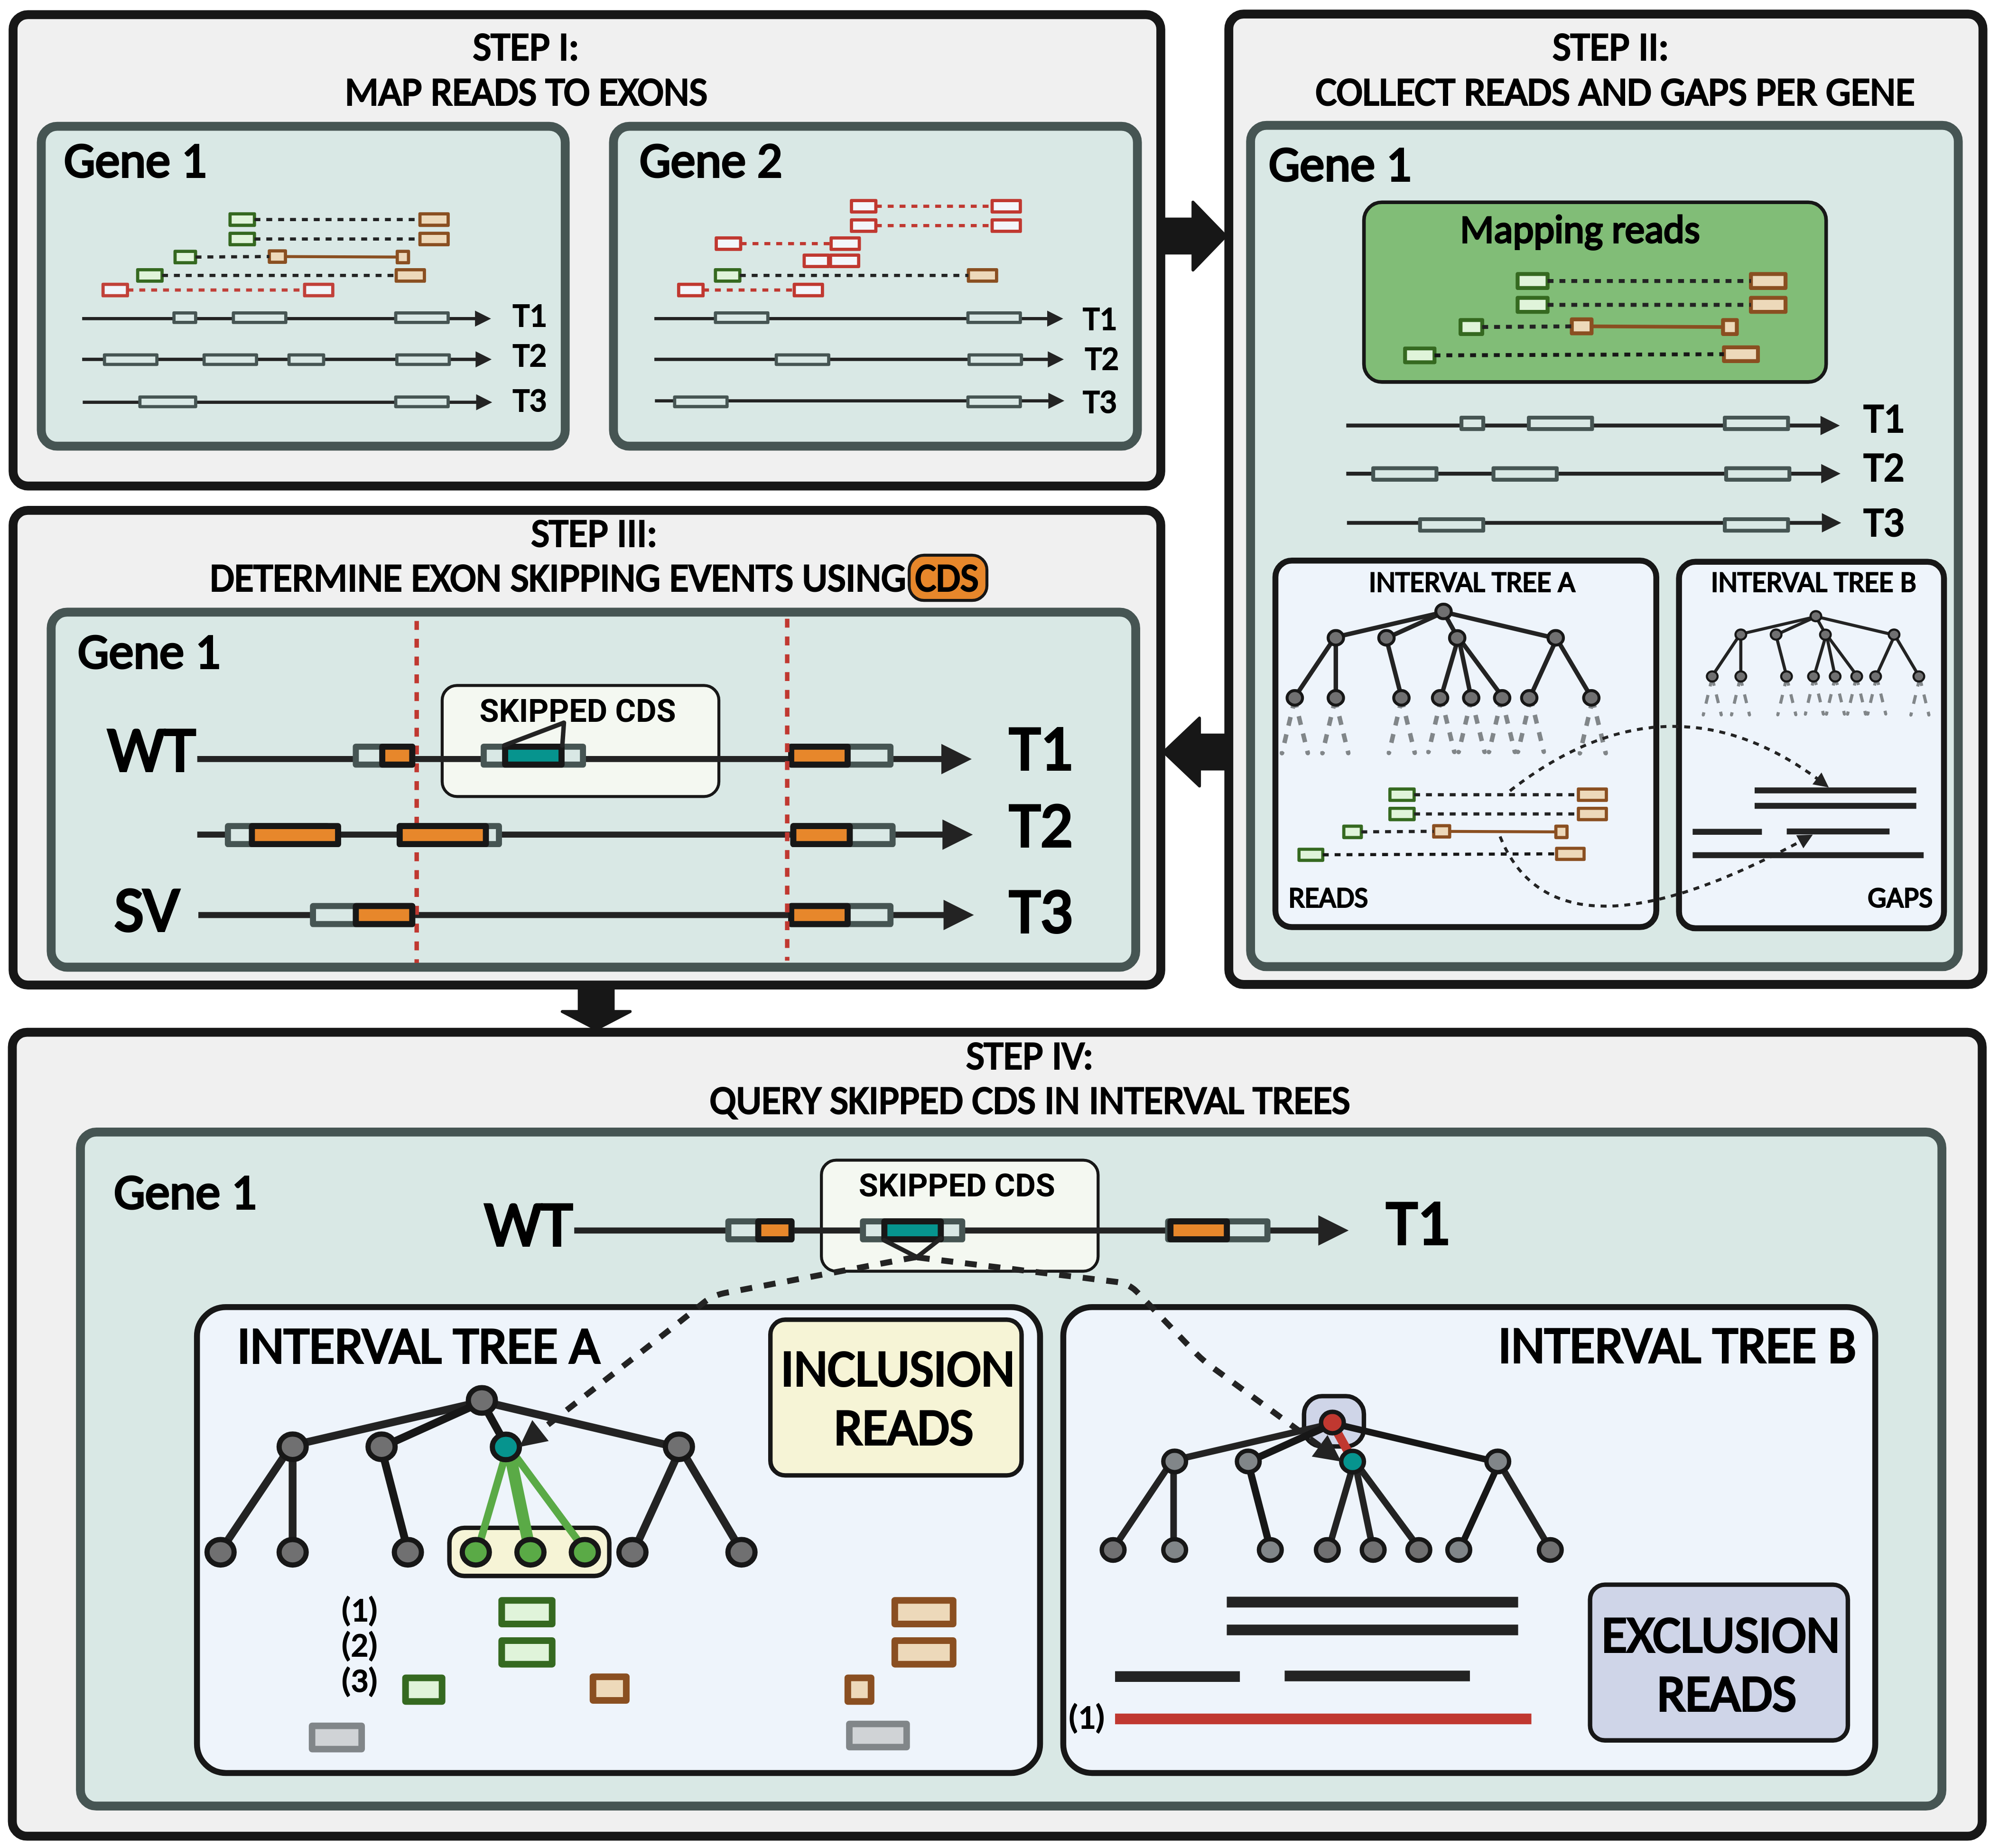
\includegraphics[width=0.99\textwidth]{./figures/PSI-Mapping.png}
    \caption{Programmlogik zur Berechnung der \textit{IRC} und \textit{ERC counts} pro \textit{Skipped Exon Event}.
    In dem Beispiel hätte das übersprungene Exon von \textbf{G1} einen \textit{PSI} Wert von 0.75.
    Die Abbildung wurde mit \cite{biorender} erstellt.}

    \label{fig:PSI-Mapping-png}
\end{figure}

Der \textit{JAR} werden eine \textit{bam}- und ein \textit{GTF}-Datei übergeben.
Zudem muss eine Ausgabedatei Spezifiziert werden:
\begin{verbatim*}
    java -jar psi.jar -bam <bam> 
                      -gtf <gtf> 
                      -o <ausgabe.psi>
\end{verbatim*}

Die \textit{JAR} liest zunächst die \textit{GTF}-Datei ein und speichert alle \textit{Gene} und deren annotierte
\textit{Transkripte} ab. 
Dabei enthält jedes \textit{Transkript} jeweils dessen \textit{Exons} \textbf{und} \textit{Coding DNA Sequences (CDS)}.
Gleichzeitig wird die \textit{bam}-Datei mittels der \textit{samtools library} decodiert und abgespeichert.
Nach der Einleseroutine kann das Programm in vier Schritte eingeteilt werden (siehe Abbildung \ref{fig:PSI-Mapping-png}):

\begin{itemize}
    \item[\textbf{I.}] \textbf{MAP READS TO EXONS}

        Die \textit{Read Pair} Koordinaten werden mit den \textit{\textbf{Exon}} Koordinaten der Transkripte abgeglichen. 
        Sobald mindestens ein \textit{Read Pair} auf ein \textit{Gen} \textit{mapped}, wird das \textit{Gen}
        in einer \textit{ArrayList<Gene> \textbf{mappedGenes}} abgelegt.
        Die Kriterien für einen validen \textit{Read} wurden bereits im letzten Report geklärt. 

    \item[\textbf{II.}] \textbf{COLLECT READS AND GAPS PER GENE}

        Für jedes der Gene in \textbf{\textit{mappedGenes}} werden nun zwei Intervalbäume $A, B$ erstellt.
        Baum $A$ beinhaltet alle \textit{AlignmentBlocks} der zum Gen zugeteilten \textit{Read Pairs},
        während Baum $B$ die Lücken zwischen einzelnen \textit{AlignmentBlocks} und zwischen
        den \textit{Forward} und \textit{Reverse Reads} abspeichert.

    \item[\textbf{III.}] \textbf{DETERMINE EXON SKIPPING EVENTS USING CDS}

        Im nächsten Schritt wird über alle Gene aus \textbf{\textit{mappedGenes}} iteriert.
        Für jedes einzelne Gen werden alle \textit{Skipped Exon Events} mittels der
        \textit{CDS} des Gens berechnet. Dabei wird dieselbe Logik wie in 
        Report 1 verwendet.

    \item[\textbf{IV.}] \textbf{QUERY SKIPPED CDS IN INTERVALTREE}

        Für jede \textit{CDS} werden nun dessen Intervalle in den Bäumen $A, B$ abgefragt und die
        \textit{Read IDs} gezählt.
        \[
        IRC := |\left\{\textit{A.\textbf{getIntervalsSpannedBy}(CDS.getStart(), CDS.getStop())}\right\}|
        \]
        \[
        ERC := |\left\{\textit{B.\textbf{getIntervalsSpanning}(CDS.getStart(), CDS.getStop())}\right\}|
        \]
        Dabei werden für $IRC$ \textbf{Intervalle} in $A$ betrachtet, \textbf{die von der \textit{CDS} überspannt werden} \\
        ($\equiv$ "\textit{Reads} die innerhalb der \textit{CDS} liegen") und für 
        $ERC$ werden \textbf{Intervalle} in $B$ gesucht, \textbf{die die \textit{CDS} überspannen} 
        ($\equiv$ "Intervalle, die die \textit{CDS} beinhalten").
\end{itemize}
\newpage

Die \textit{PSI} Werte werden in die Ausgabedatei mit folgendem Format geschrieben:
\begin{verbatim*}
   Gene ID            cdsStart-cdsStop   IRC   ERC  Total  PSI
   ENSG00000165623.5  13275735-13275801  25    13   38     0.65
   ...                ...                ...   ...  ...    ...
\end{verbatim*}

\section{Hypothesen Test}
Wir wollen untersuchen, ob der Prozess des \textit{Alternativen Splei\ss ens} anhand von 
\textit{Exon Skipping Events} ($\mathbf{\Psi}$) rein zufällig stattfindet, oder von regulatorischen 
Mechanismen gesteuert wird. 

\begin{itemize}
    \item \textbf{H\textsubscript{0}} := \textit{Exon Skipping Events} finden zufällig statt.
    \item \textbf{H\textsubscript{1}} := \textit{Exon Skipping Events} sind nicht reiner Zufall.
\end{itemize}
Dafür nehmen wir an, dass die Anzahl an \textit{IRC} Binomial Verteilt ist:

\[
P(i,N|p) = \binom{N}{i}p^{i}(1-p)^{N-i}
.\]
Hierbei beschreibt $p$ die Wahrscheinlichkeit, dass ein einzelnes \textit{Exon} als \textit{Inclusion Read} klassifiziert wird,
während $N$ die Anzahl an \textit{Reads} darstellt, die für das momentane \textit{Exon} einen Informationsgehalt haben.
Zudem gehen wir davon aus, dass jedes Transkript mindestens einen informativen \textit{Read} pro Exon hat.

Für den Test wurden die zehn Ausgabedateien der \textit{JAR} in zwei Gruppen unterteilt (siehe Tabelle \ref{tab:einteilung}):

\begin{table}[htpb]
    \centering
    \caption{Einteilung der Samples in zwei Gruppen}
    \label{tab:einteilung}
\begin{tabular}{|l||c|c|c|c|c|c|c|c|c|c|} \hline
     Ausgabedatei $i$   & 1 & 2 & 3 & 4 & 5 & 6 & 7 & 8 & 9 & 10 \\\hline
     Gruppe $g_{i}$ & 1 & 1 & 1 & 1 & 1 & 2 & 2 & 2 & 2 & 2 \\\hline
     IRC          &$i_{1}$&$i_{2}$&$i_{3}$&$i_{4}$&$i_{5}$&$i_{6}$&$i_{7}$&$i_{8}$&$i_{9}$&$i_{10}$  \\\hline
     Gesamt Anzahl&$N_{1}$&$N_{2}$&$N_{3}$&$N_{4}$&$N_{5}$&$N_{6}$&$N_{7}$&$N_{8}$&$N_{9}$&$N_{10}$  \\ \hline\hline
     $\mathbf{\Psi_{reduced}} \sim (p_{0})$   &$p_{0}$&$p_{0}$&$p_{0}$&$p_{0}$&$p_{0}$&$p_{0}$&$p_{0}$&$p_{0}$&$p_{0}$&$p_{0}$\\\hline
     $\mathbf{\Psi_{full}} \sim  (p_{1}, p_{2})$ &$p_{1}$&$p_{1}$&$p_{1}$&$p_{1}$&$p_{1}$&$p_{2}$&$p_{2}$&$p_{2}$&$p_{2}$&$p_{2}$\\\hline
\end{tabular}
\end{table}
\newpage

Dabei simulieren wir zwei \textit{Modellen}:
\begin{itemize}
    \item $\mathbf{\Psi_{reduced}} \sim(p_{0})$: Hat einen einzigen Parameter $p_{0}$ für alle Gruppen.
    \item $\mathbf{\Psi_{full}} \sim(p_{1}, p_{2})$: Besitzt zwei verschiedenen Parameter.
\end{itemize}

Die \textit{Likelihood} kann nun mit der \textit{Maximum Likelihood Estimation} Methode
abgeschätzt werden.
Die \textit{Likelihood Funktionen} lasses sich wie folgt definieren:
\begin{itemize}
    \item $\mathbf{L_{reduced}(p_{0})} := \prod_{j = 1}^{10}P(i_{j},N_{j}|p_{0})$
    \item $\mathbf{L_{full}(p_{1}, p_{2})} := \prod_{j = 1}^{10}P(i_{j},N_{j}|p_{g_{j}})$
\end{itemize}


\section{Vergleich mit DEXSeq}
% ------------------------------------------------------------------------------





% ------------------------------------------------------------------------------
% \printbibliography
% ------------------------------------------------------------------------------


% ------------------------------------------------------------------------------
\newpage~\appendix
% ------------------------------------------------------------------------------

\section{Appendix Section}

hm 

Text goes here



\end{document}
